% A good introduction to latex can be found here:
%    http://www.cse.ohio-state.edu/~hank/latex/lshort141.pdf

\documentclass{article}

\usepackage{full page}  % make the margins somewhat smaller than the default

\usepackage{listings}  %  needed for source code listings
\usepackage{color}
\definecolor{dkgreen}{rgb}{0,0.6,0}
\definecolor{gray}{rgb}{0.5,0.5,0.5}
\definecolor{mauve}{rgb}{0.58,0,0.82}

\lstset{frame=tb,
  language=Java,
  aboveskip=3mm,
  belowskip=3mm,
  showstringspaces=false,
  columns=flexible,
  basicstyle={\small\ttfamily},
  numbers=left,
  numberstyle=\tiny\color{gray},
  keywordstyle=\color{blue},
  commentstyle=\color{dkgreen},
  stringstyle=\color{mauve},
  breaklines=true,
  breakatwhitespace=true
  tabsize=3
} 

\usepackage{graphicx}        

% set the document title, author, and date here.
%  once set, the \maketitle command (within the document)
%  will display them nicely
\title{Dartmouth Campus Guide Report}
\author{Tianlong Yun, Xiaohong Qiu, Mengjia Kong}

\begin{document}
\maketitle

\section{Introduction}
We have made a campus tour guide. Unlike the other existing tour guides, our app is community-based, just as the way wiki does. Each user is able to contribute his interested place into a shared centralized repository, which is maintained by a central server. User has access to all the current available places recommended by others and provide comments if he wants. If a place is not in the repository and other users might be interested in it, user can create a new entry for the place. The new entry includes name and a short text description. User has the option to take a couple of pictures for the place. User also can record an audio which provides a simple voice introduction about the place. Moreover, a ranking ranging from 1 to 5 can be selected for that place. Once user clicks the save button, all the information about the new place will be stored into local and server database concurrently.

Our backend server serves as a centralized agent to manipulate all the places currently available in the repository. Everyone is able to view all the places recommended by others via browser. However, only administrator has the privilege to delete a specific place. Plus we have deployed our server into Google cloud and thus got a domain name. So the user can just only download the android app and install it. Then they can play with it.


\section{Architectural Design}
\subsection{OO design diagram}
Our OO diagram of android app is in Figure \ref{F:campuswiki}. Our 00 diagram of server is in Figure \ref{F:campuswiki_server}.

\begin{figure}[h!]   
\centering
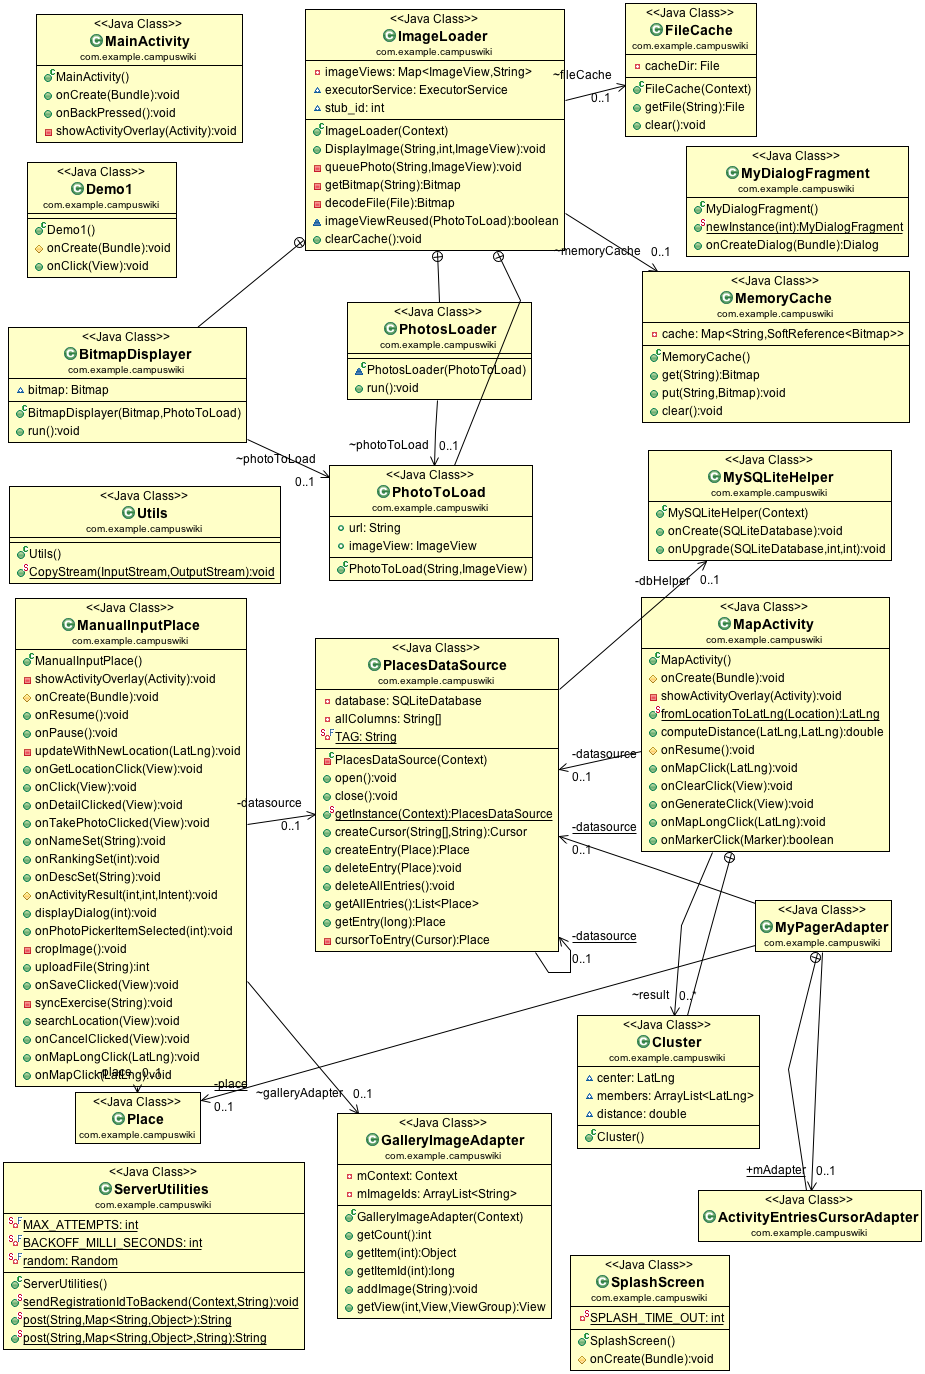
\includegraphics[width = 300pt]{Figures/CampusWiki_2.png}
\caption{Dartmouth Campus Guide App Design Diagram}
\label{F:campuswiki}
\end{figure}



\begin{figure}[h!]   
\centering
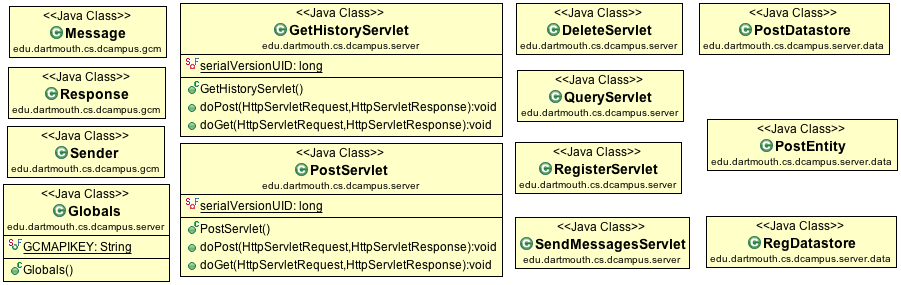
\includegraphics[width = 300pt]{Figures/server_diagram.png}
\caption{Dartmouth Campus Guide Server Design Diagram}
\label{F:campuswiki_server}
\end{figure}

\subsection {class descriptions}

\subsubsection{Client}

\begin{itemize}
\item 
\verb`ManualInputPlace.java`:
The class is used to create a new entry for a place. It shows a couple of buttons to perform various functions. Using these buttons, user can record an audio to provide a voice introduction, take a couple of pictures to represent the place, obtain GPS location on Google map. The taken pictures and recorded audios will be stored into web storage server. The database can just stores their URLs. User can also select a ranking level for the place. Once save button is clicked, all the information will be stored into local and server database.

\item
\verb`MyPageAdapter.java`:
It is subclass of PageAdapter and has two pages. One page is listview of all the places in the local database. If user clicks Sync, then the local database will be cleared first and all the places in server will be populated into the local database and automatically populate listview. The other page is a detailed presentation of a certain place. All the pictures associated with the place will show up and can be swiped horizontally. Then a ranking bar will appear below the pictures. Underneath is a Google map with GPS location indicated by a marker. Below that is voice introduction you can play and stop it any time. The bottom is a text description of the place followed by all comments posted by all users.

\item
\verb`Place.java`: 
This is a bean holding all the attributes associated with a place including name, latlng, pictures, ranking, voice audio, text description, ranking etc.

\item
\verb`PlaceDataStore.java`:
This class provides a wrapper for SQLite related operations such as createEntry(), deleteEntry(), deleteAll(), query(), queryAll() etc.

\item
\verb`ServerUtilites.java`:
This class provides a wrapper for various operations on java URL connections. The most import one is post(), which is used to send requests and json-fomatted data to server.

\item
\verb`MyDialogFragment.java`:
This class provides centralized helper functions to handle all kinds of dialogs used in the app, such as when taking a picture, when prompting for text or when clicking recording stop.

\item
\verb`Utils.java MemoryCache.java ImageLoader.java FileCache.java`:
These class will download audio and pictures from server, and cache them.

\item
\verb`SplashScreen.java`:
This class provides a thread to handle the fade in and fade out of the splash screen.

\item
\verb`PlacesDataSource.java MySQLiteHelper.java`:
These two class are helper class which provide you with the routines to manipulate the SQLite datasource, including add, delete or query.

\item
\verb`MapActivity.java`:
This class will show the map of Dartmouth, and visual all the pre-existing locations and locations by the users. User could click on the place balloon to view the detail or they can also long click on some point to and a new entry. 

\item
\verb`MainAvtivity.java`:
This class will initialize the page adapter.

\item
\verb`Demo1.java`:
The class contains routine to show the transparent activity.

\item
\verb`GalleryImageAdapter.java`:
This class will handle the routine for show the gallery and enlarged view of pictures


\end{itemize}


\subsubsection{Server}
There are two parts classes in server: Backend and Frontend. Frontend is about the webpage which will be present in a browser. Backend can also be split into two parts, webpage backend and datastore.

\begin{itemize}
\item 
\verb`QueryServlet.java`:
This class queries all data items in datastore. There are two methods \lq\lq \verb`doPost`\rq\rq and \lq\lq \verb`doGet`\rq\rq  ~in this class with same function.

\item
\verb`PostServlet.java`:
This class is to add a new data to datastore. There are two methods \lq\lq \verb`doPost`\rq\rq and \lq\lq \verb`doGet`\rq\rq  ~in this class with same function.

\item
\verb`DeleteServlet.java`:
This class is to delete a data from datastore and refresh the webpage. There are two methods \lq\lq \verb`doPost`\rq\rq and \lq\lq \verb`doGet`\rq\rq  ~in this class with same function.

\item
\verb`GetHistoryServlet.java`:
This class is to query all data items in datastore and send them to device. There are two methods \lq\lq \verb`doPost`\rq\rq and \lq\lq \verb`doGet`\rq\rq  ~in this class with same function.

\item
\verb`RegisterServlet.java`:
This class is to register a new device to server and store the information of this device in register datastore. There are two methods \lq\lq \verb`doPost`\rq\rq and \lq\lq \verb`doGet`\rq\rq  ~in this class with same function.

\item
\verb`PostEntity.java`:
This class is about the data structure which is stored in datastore. Only structure method in this class.

\item
\verb`PostDatastore.java`:
This class is about the DatastoreService which provides a datastore to store all location informations in this project. \lq\lq \verb`add`\rq\rq ~method is to add a new data to this datastore. \lq\lq \verb`query`\rq\rq ~is to get all data in datastore in the type of \verb`PostEntity`. \lq\lq \verb`delete`\rq\rq ~is to delete the specific data in the datastore. 

\item
\verb`RegDatastore.java`:
This class is about the DatastoreService which provides a datastore to store all information of devices in this project. \lq\lq \verb`register`\rq\rq ~is to add a new device item to this datastore. \lq\lq \verb`getDevices`\rq\rq ~is to get all devices from datastore.

\item
\verb`main.jsp`:
This file is not a class but a jsp file about the webpage, which builds from html, java, css, jQuery.


\end{itemize}

\section{How to run the demo}
\subsection{Client}

\begin{enumerate}
\item
First Start the Server in RealCloud, or just use ours: http://dartcampuswiki.appspot.com/

\item
Change the IP address of the string value at App side to the IP address e.g. http://dartcampuswiki.appspot.com/

\item
Run
\end{enumerate}


\subsection{Server}
We have run the server on the real Cloud. The url is http://dartcampuswiki.appspot.com . 
The resources are also provided in the svn, which can be import into your eclipse and run in your own computer. The steps of running the project on the real cloud is :
\begin{enumerate}
\item 
Import the existing project in your workspace of eclipse. Maybe there are some bugs according to the environment. According to my experience, the Google App Engine SDK may be missing. Then a specific Google App Engine SDK need to be added.

\item
Press run, you can see the server on http://localhost:8888 .

\item
To run in the real cloud, we use Google App Engine. Create an application on Google App Engine's Application Overview and set the Application Identifier and Title. Next, deploy the project in eclipse to the app engine. Finally, you can see the server on the real cloud when you open the \"application identifier.appspot.com\" in a browser! The details is exactly like the lecture notes in cs65 course website.

\end{enumerate}

\section{Demo}
When you start our app on a android phone, users will see splash screen in Figure \ref{F:splash}.

\begin{figure}[h!]
\begin{minipage}[h!]{0.3\linewidth}
\centering
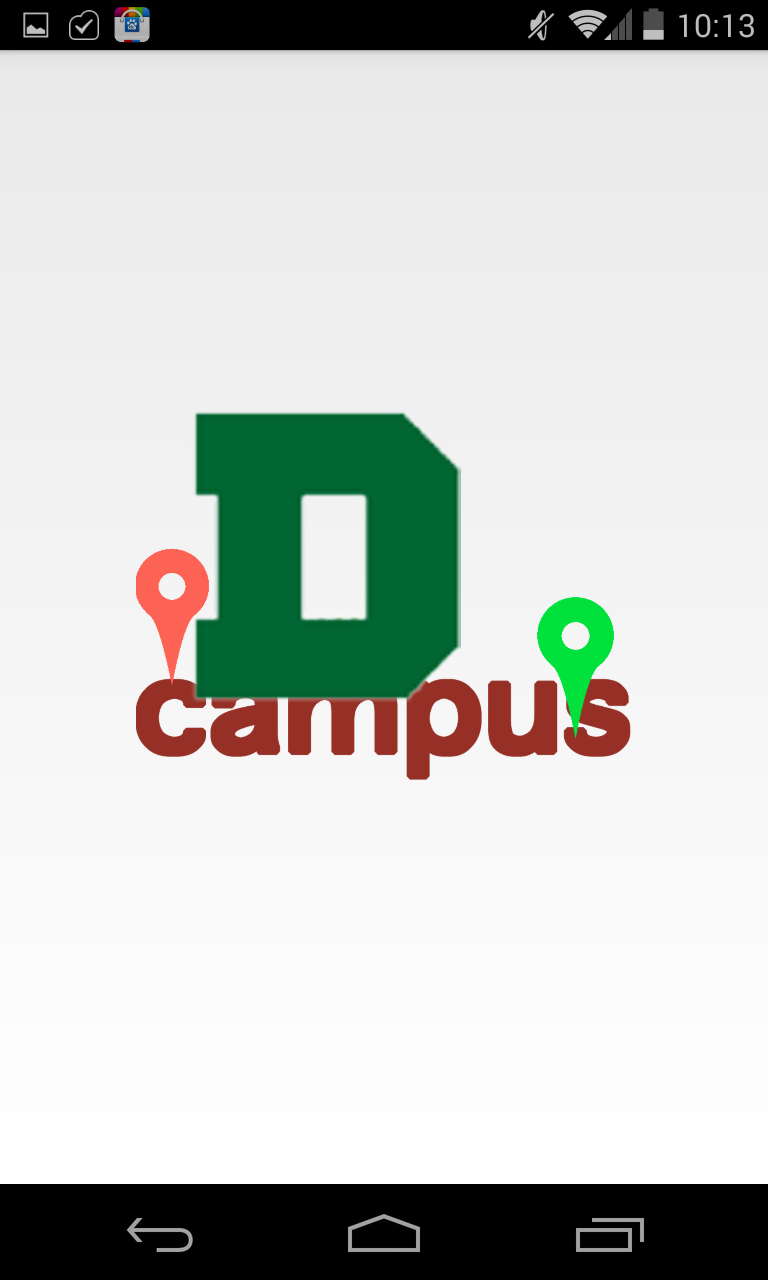
\includegraphics[width=1.5in]{figures/splash_screen.png}
\caption{Splash Screen}
\label{F:splash}
\end{minipage}%
\begin{minipage}[h!]{0.4\linewidth}
\centering
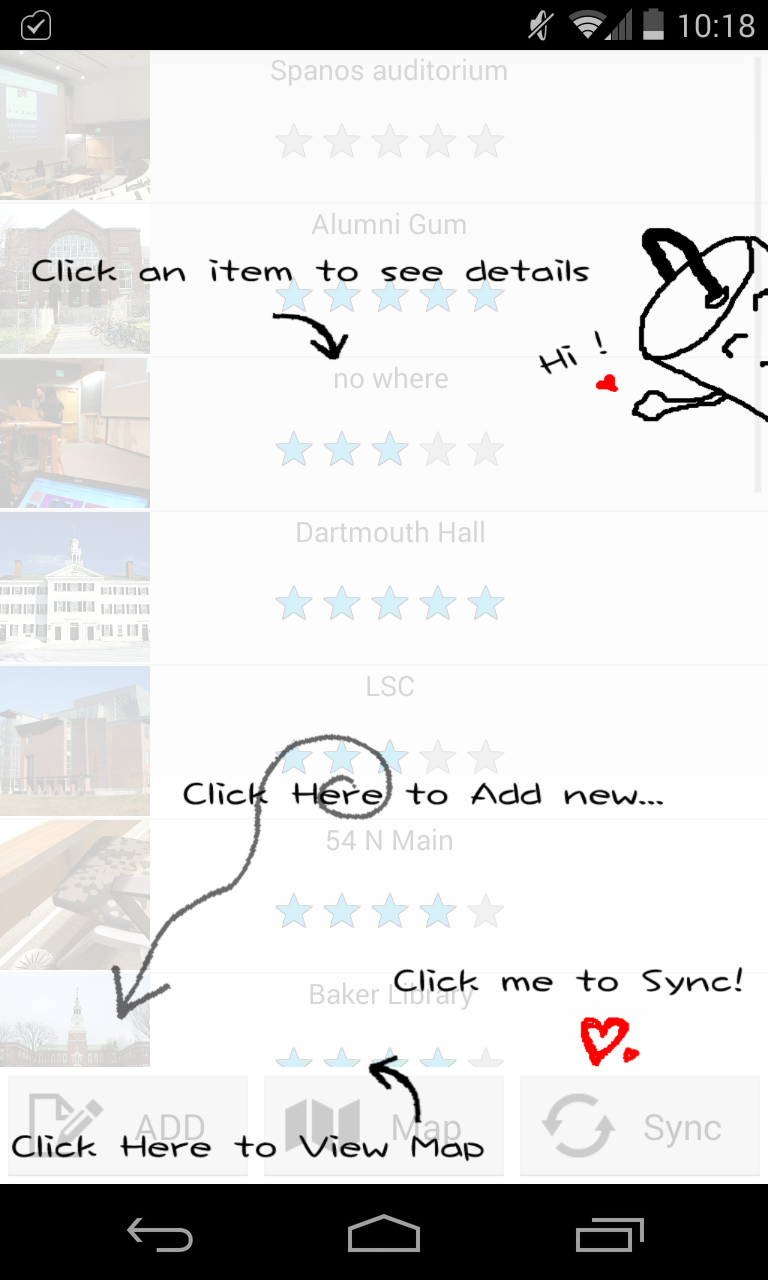
\includegraphics[width=1.5in]{figures/main_view_intro.png}
\caption{Introduct how to use main view}
\label{F:main_view_intro}
\end{minipage}
\begin{minipage}[h!]{0.3\linewidth}
\centering
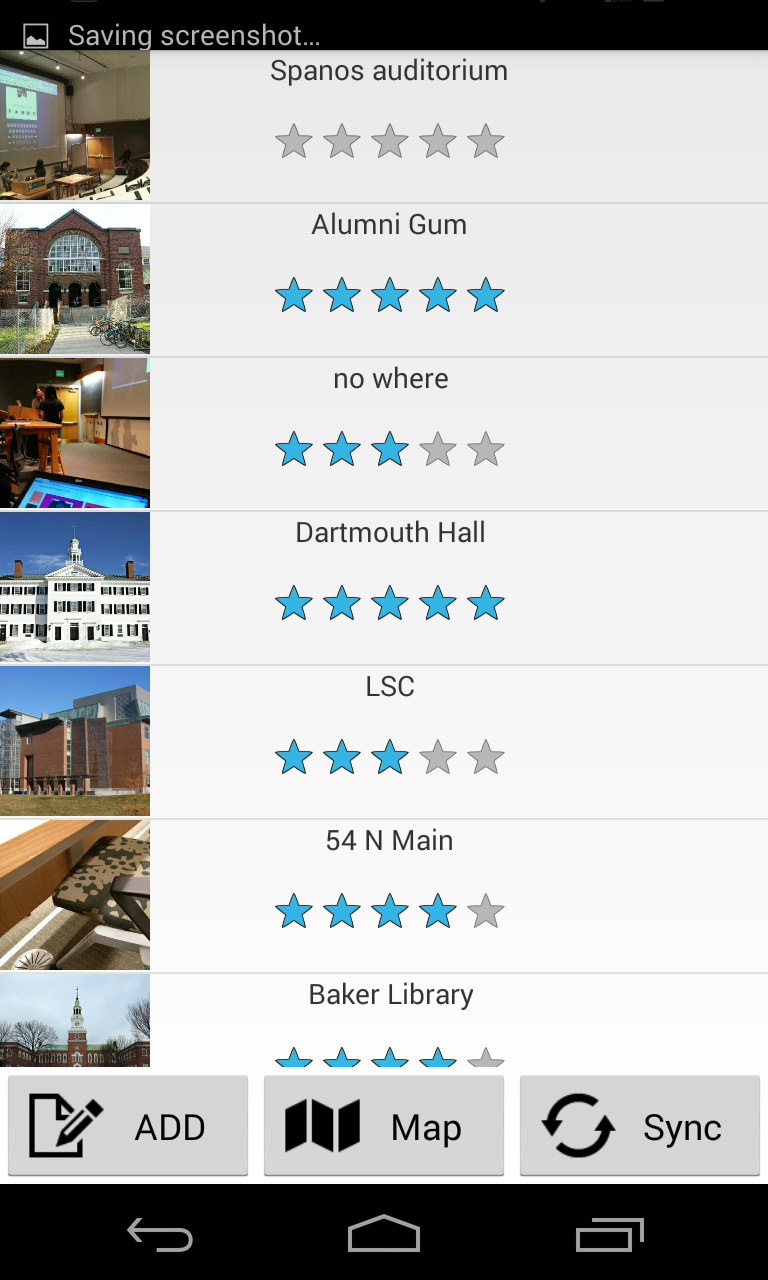
\includegraphics[width=1.5in]{figures/main_view.png}
\caption{Main View}
\label{F:main_view}
\end{minipage}%
\end{figure}

When the app downloading succeeds, users will see a introduction of how to use the main view like Figure \ref{F:main_view_intro}. Touch anywhere then the main view will show up in Figure \ref{F:main_view}. Press any item, uses can see the details of this item in Figure \ref{F:item}.

Press Add button, users will see a introduction of how to use the add view like Figure \ref{F:add_intro}. Touch anywhere then the add view will show up in Figure \ref{F:add}.

\begin{figure}[h!]
\begin{minipage}[h!]{0.3\linewidth}
\centering
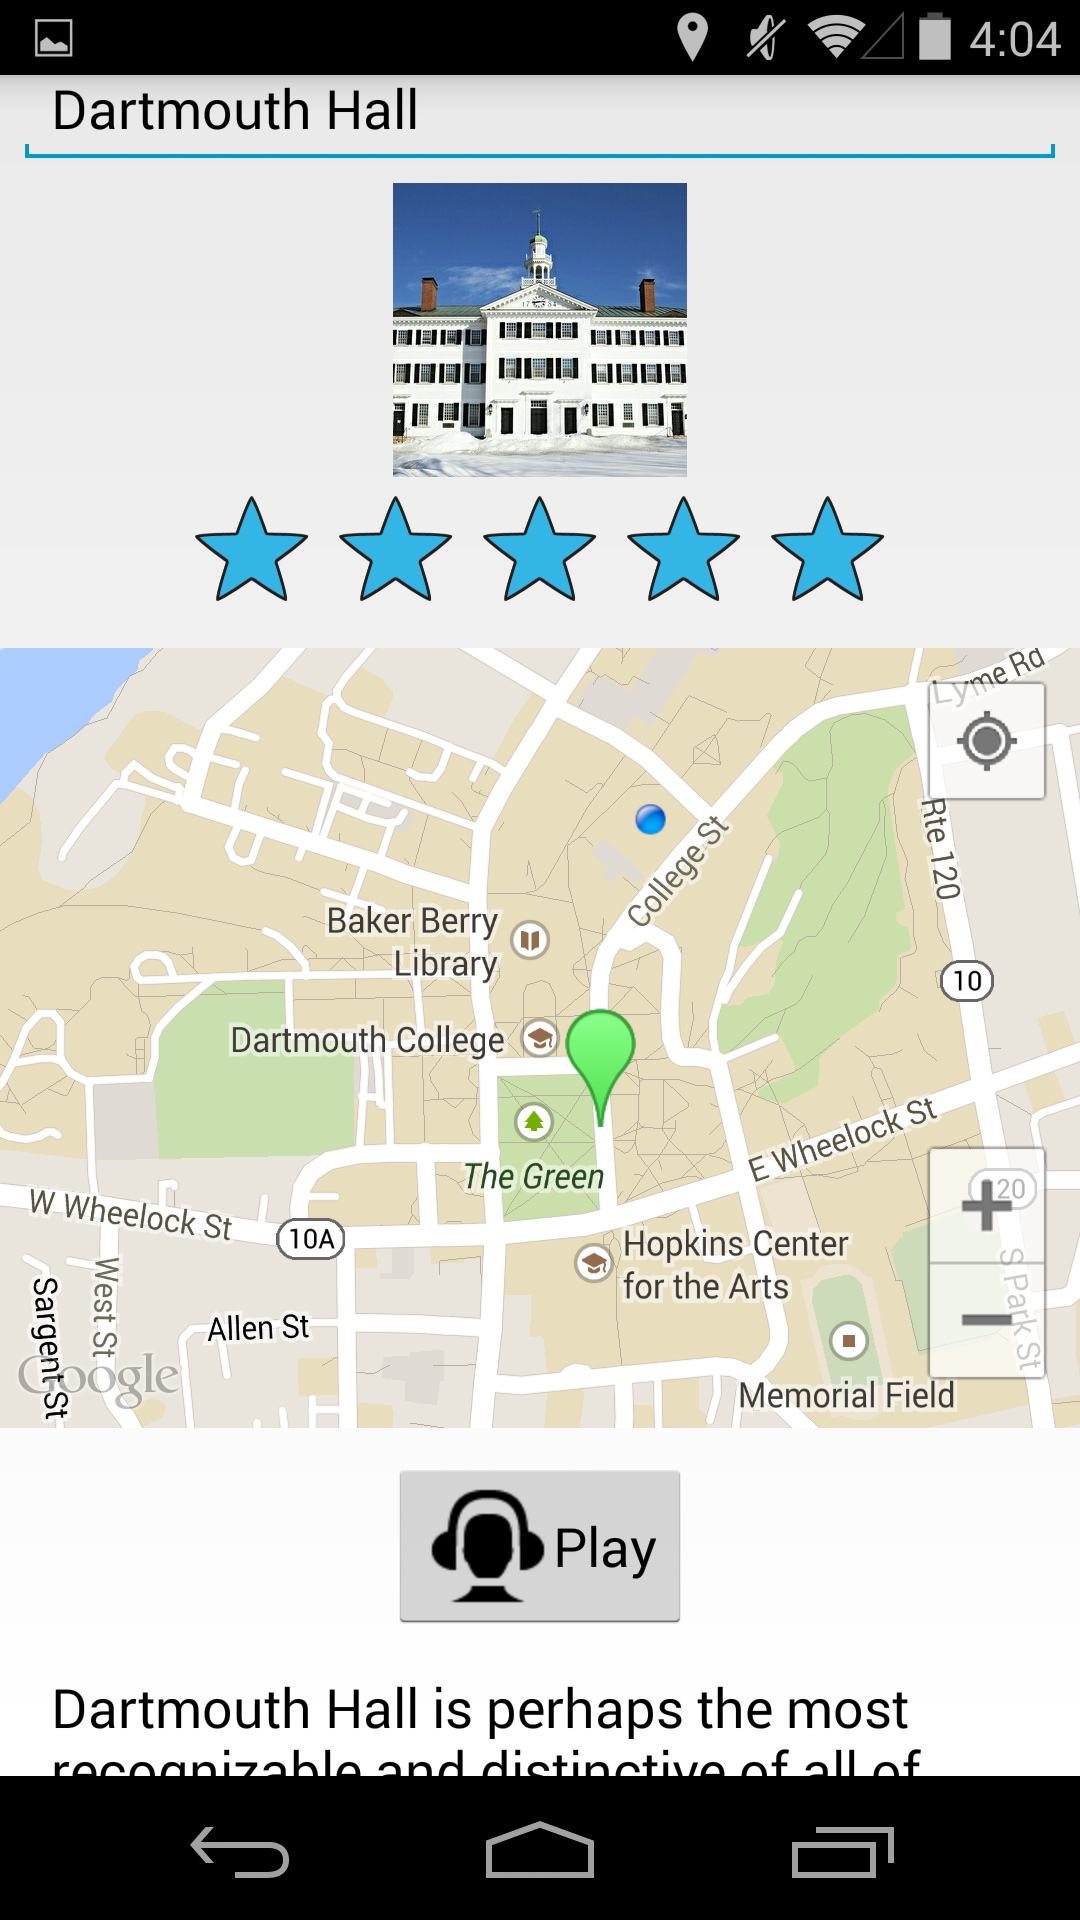
\includegraphics[width=1.5in]{figures/item.png}
\caption{Details of Dartmouth Hall}
\label{F:item}
\end{minipage}
\begin{minipage}[h!]{0.4\linewidth}
\centering
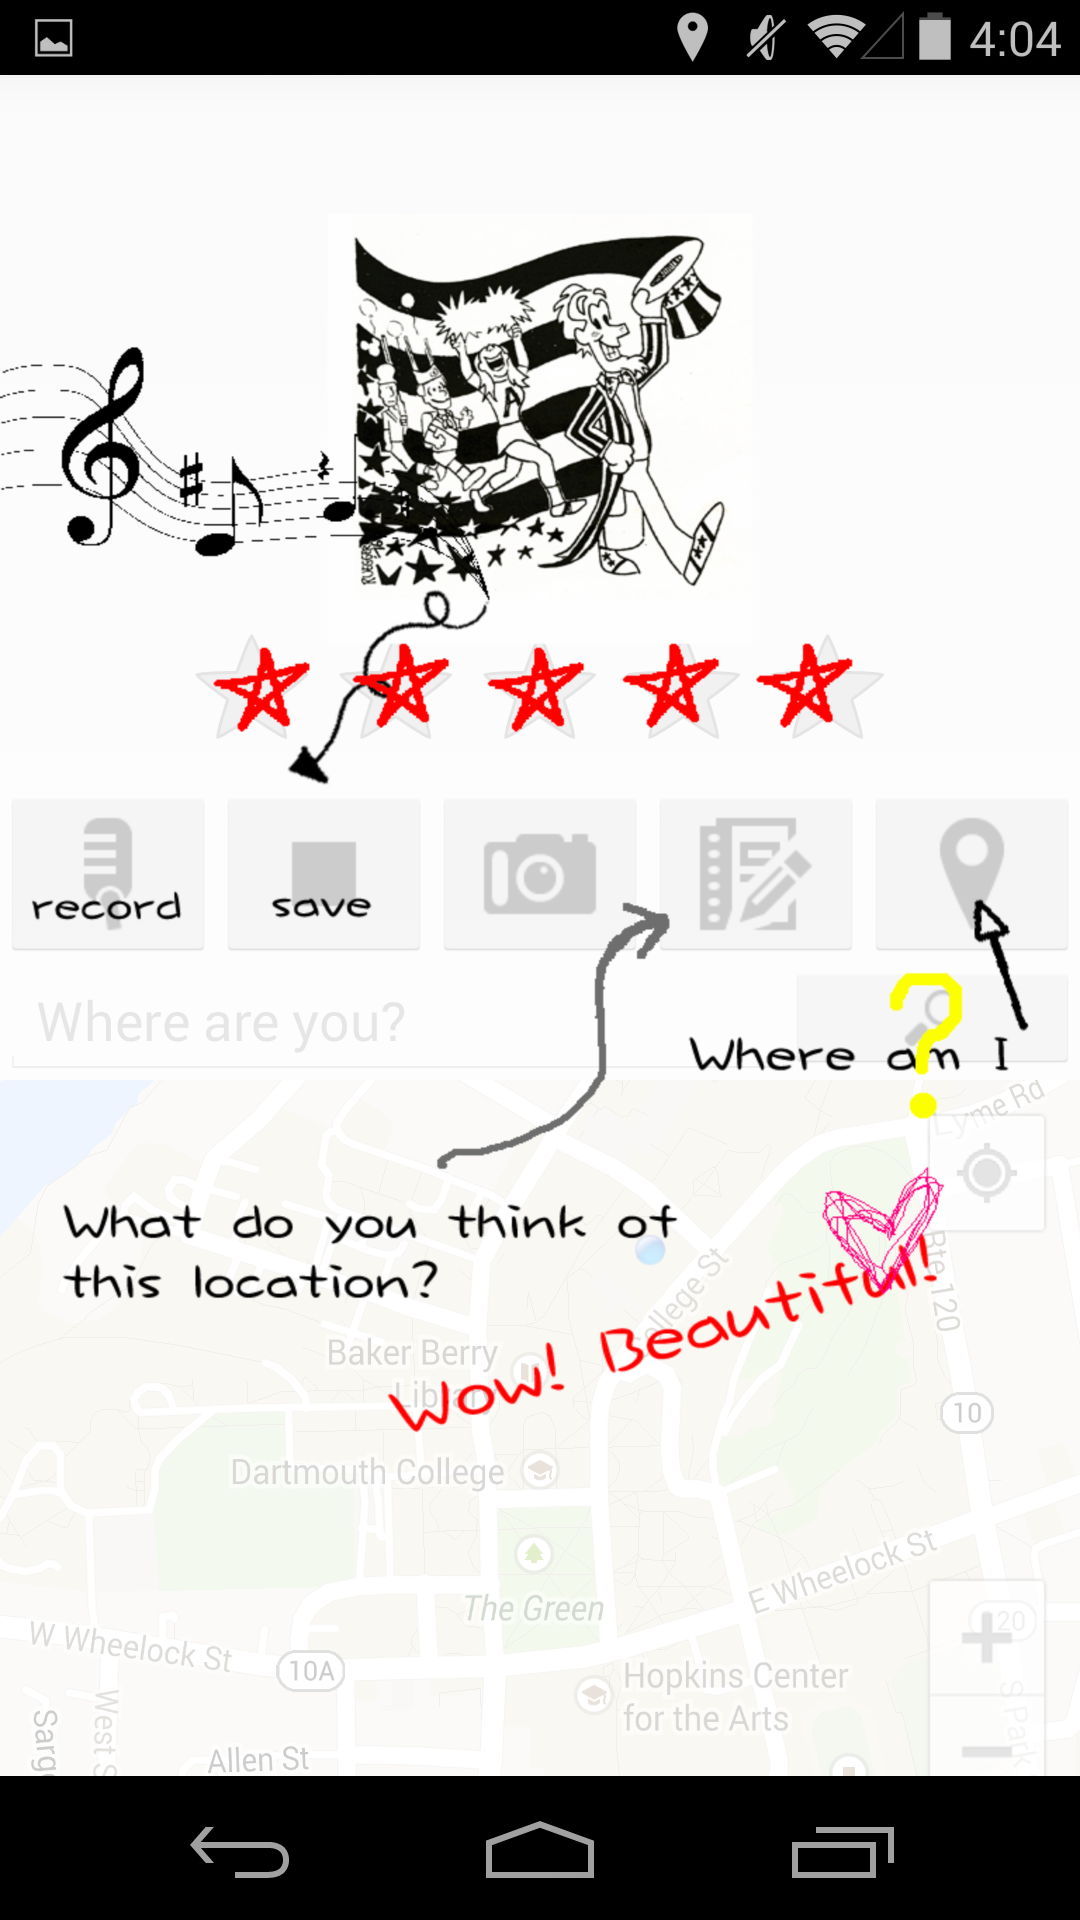
\includegraphics[width=1.5in]{figures/add_intro.png}
\caption{Introduct the add view}
\label{F:add_intro}
\end{minipage}%
\begin{minipage}[h!]{0.3\linewidth}
\centering
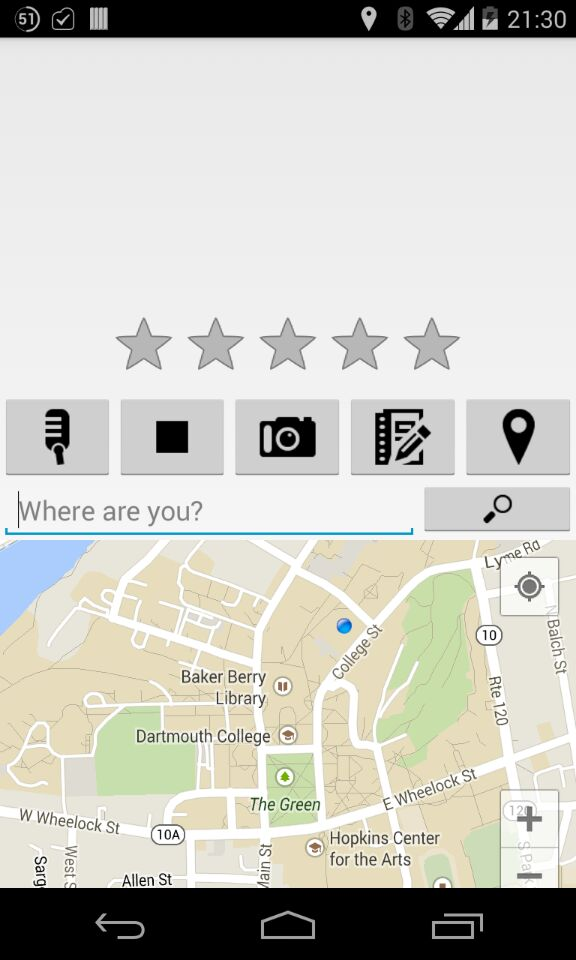
\includegraphics[width=1.5in]{figures/add.jpg}
\caption{Add View}
\label{F:add}
\end{minipage}
\end{figure}



In main view, press Map button, users will see a introduction of how to swipe between views like Figure \ref{F:swipe}. Touch anywhere then the map view will show up in Figure \ref{F:map}.

\begin{figure}[h!]
\begin{minipage}[h!]{0.5\linewidth}
\centering
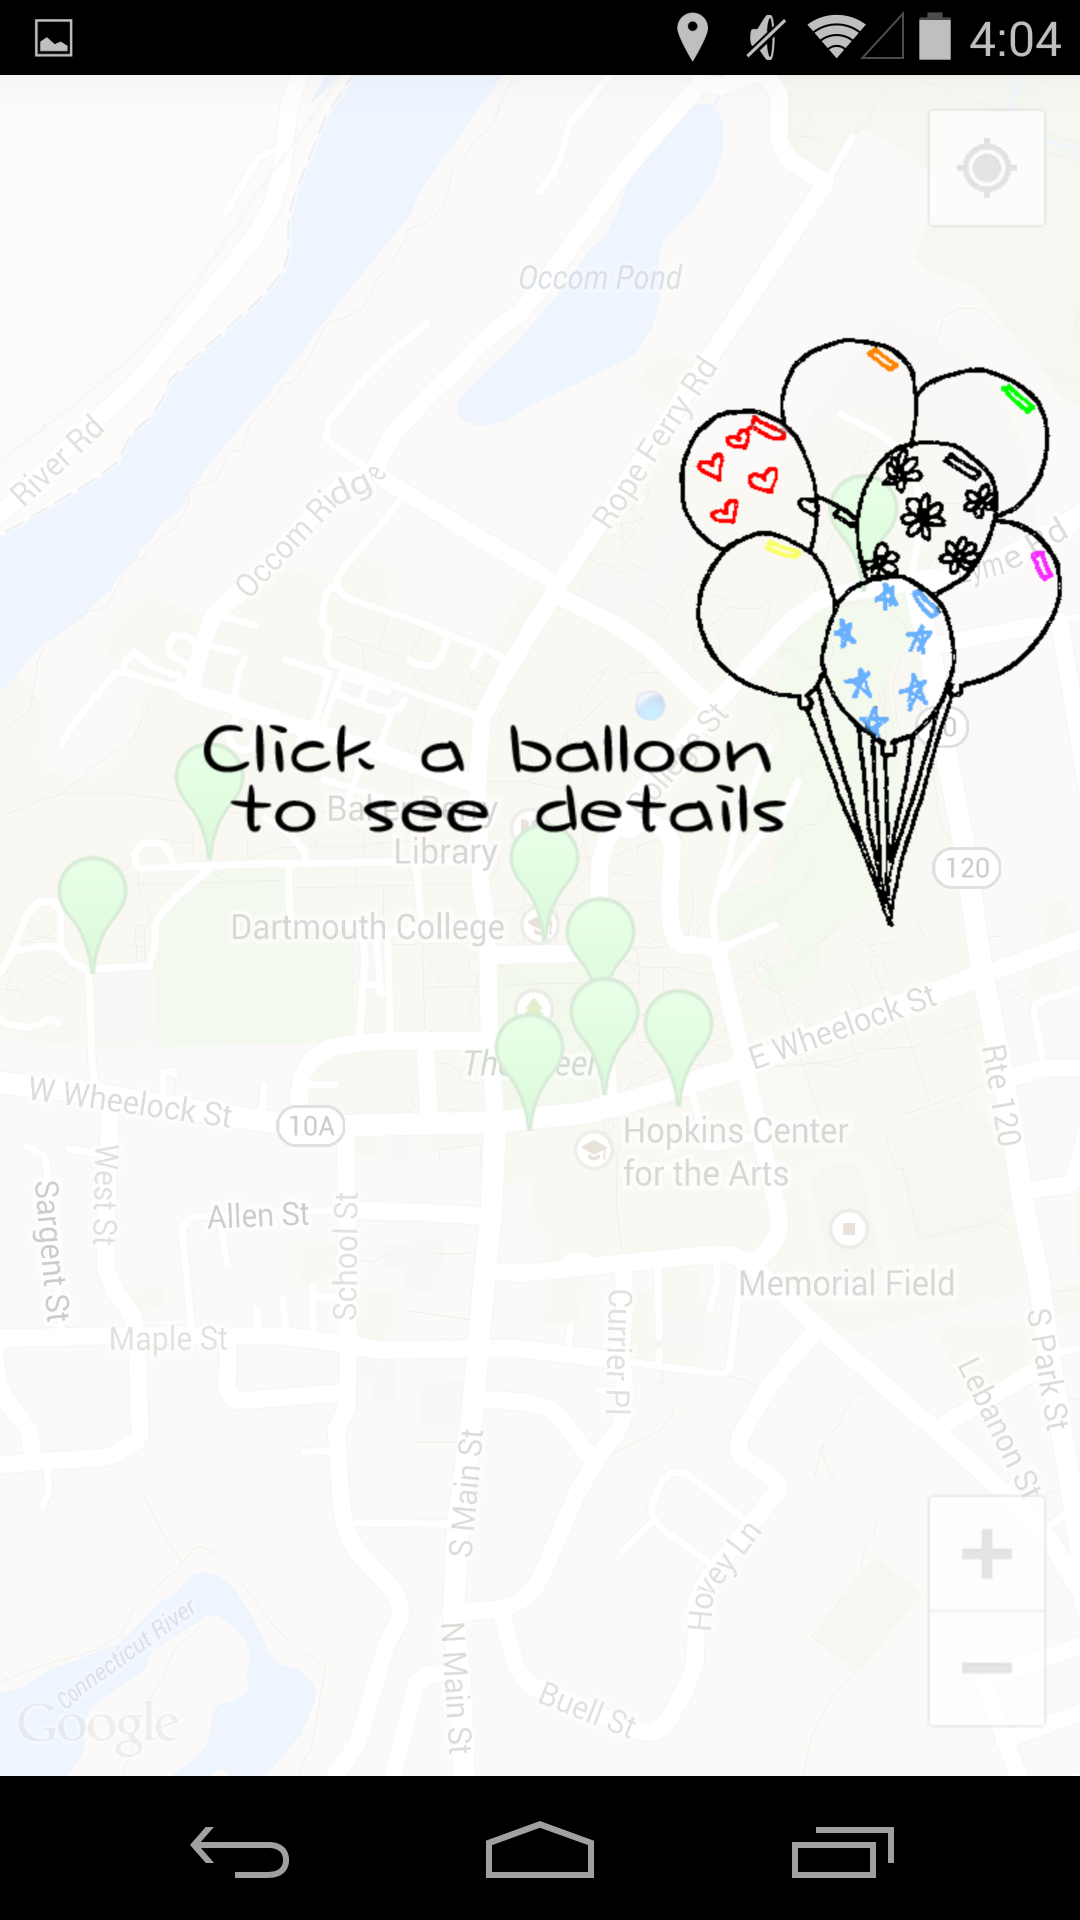
\includegraphics[width=1.5in]{figures/map_intro.png}
\caption{Introduct the swipe function}
\label{F:swipe}
\end{minipage}%
\begin{minipage}[h!]{0.5\linewidth}
\centering

\includegraphics[width=1.5in]{figures/map.png}
\caption{Map View}
\label{F:map}
\end{minipage}
\end{figure}

Users also can see locations in a website: http://dartcampuswiki.appspot.com/ . The view is in Figure \ref{F:server}.

\begin{figure}[h!]   
\centering
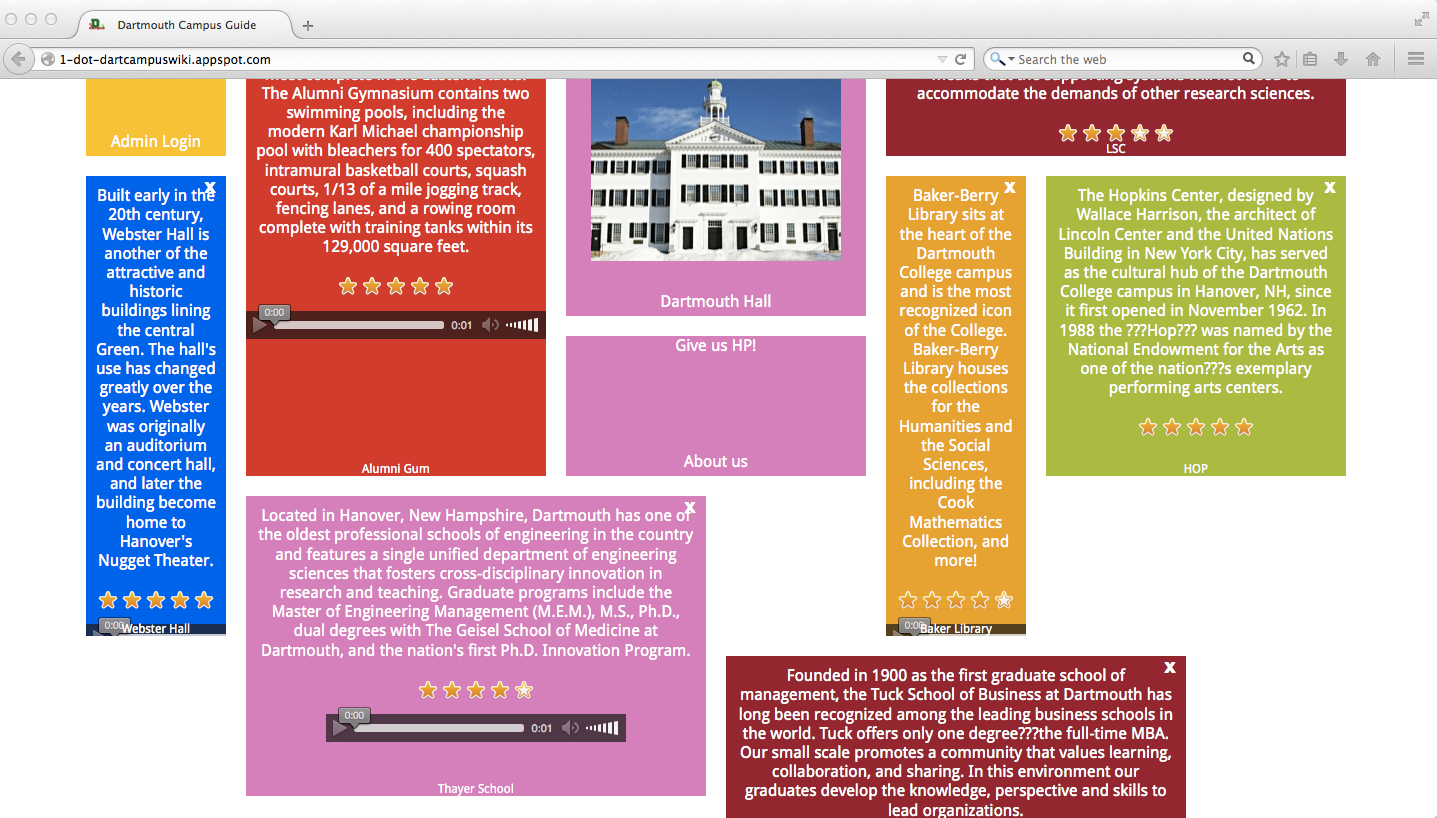
\includegraphics[width = 300pt]{Figures/server.png}
\caption{Dartmouth Campus Guide Website}
\label{F:server}
\end{figure}

\section{Lessons Learnt}
In this project, we have used many functions which we learned from classes: Widgets of UI, Camera, Compressing images, Album, Database, Map, Google app engine, Cloud. Besides, we have some innovative ideas in this project: upload and download images and audios to server.

In the progress, we have run into many problems. Once, we want to use socket to upload files to server. But Google App Engine blocks \verb`IOStream` to forbidden users to access this method. After trying variety of possible methods, we run website on Google App Engine but upload files to another server, from which both app and website get files.

Luckily, we went through all this problems finally. When these difficulties show up, many methods are tried to figure out them. There are some resources help us a lot: Stack Overflow and Android Developer. Furthermore, communicate more with TAs which will give you many feedbacks about the project.

\section{Conclusion}
One of the biggest advantages our campus tour guide over others existing ones is that it is driven and contributed by each user. Our app has deeper interaction with user and thus can better reflect and meet user needs. We use GPS and Google map as well as audio to supply a more vivid description of places. On server side, we employ two-level permission labels to manipulate the current places to avoid mal-behaviors or careless operations.

Next step is to integrate video into the app. The video should give a more vivid introduction about the place. Another improvement is if user arrives at a certain place, the corresponding audio and video should pop up once the option has been enabled. We may also consider applying our app to a broader community than campus, such as town or city or even state.


\end{document}